\documentclass[oneside,14pt]{extarticle}
\usepackage{cmap}
\usepackage[utf8]{inputenc}
\usepackage{longtable}
\usepackage[english,ukrainian]{babel}
\usepackage{graphicx}
\usepackage{geometry}
\usepackage{listings}
\usepackage{float}
\usepackage{amsmath}
\usepackage{subfig}
\usepackage{tempora}
\renewcommand{\arraystretch}{1.5}
\usepackage{mwe}
\geometry{
	a4paper,
	left=20mm,
	right=20mm,
	top=15mm,
	bottom=15mm,
}
\lstset{
	language=c,
	tabsize=4,
	keepspaces,
	showstringspaces=false,
	frame=single,
	breaklines,
	language=C,
}
\graphicspath{ {./pictures} }
\setlength{\parindent}{4em}

\newcommand\subject{Архітектура і проєктування програмного забезпечення}
\newcommand\lecturer{доцент кафедри ПЗ\\Фоменко А.В.}
\newcommand\teacher{старший викладач кафедри ПЗ\\Шкраб Р.Р.}
\newcommand\mygroup{ПЗ-42}
\newcommand\lab{6}
\newcommand\theme{Використання структурних патернів}
\newcommand\purpose{Ознайомитися з основними шаблонами проектування, навчитися застосовувати їх при проектуванні і розробці ПЗ}

\begin{document}
\begin{normalsize}
	\begin{titlepage}
		\thispagestyle{empty}
		\begin{center}
			\textbf{МІНІСТЕРСТВО ОСВІТИ І НАУКИ УКРАЇНИ\\
				НАЦІОНАЛЬНИЙ УНІВЕРСИТЕТ "ЛЬВІВСЬКА ПОЛІТЕХНІКА"}
		\end{center}
		\begin{flushright}
			\textbf{ІКНІ}\\
			Кафедра \textbf{ПЗ}
		\end{flushright}
		\vspace{80pt}
		\begin{center}
			\textbf{ЗВІТ}\\
			\vspace{10pt}
			до лабораторної роботи № \lab\\
			\textbf{на тему}: <<\textit{\theme}>>\\
			\textbf{з дисципліни}: <<\subject>>
		\end{center}
		\vspace{80pt}
		\begin{flushright}
			
			\textbf{Лектор}:\\
			\lecturer\\
			\vspace{28pt}
			\textbf{Виконав}:\\
			
			студенти групи \mygroup\\
			Коваленко Д.М.\\
			Снісар В.І.\\
			Баран В.Б.\\
			\vspace{28pt}
			\textbf{Прийняла}:\\
			
			\teacher\\
			
			\vspace{28pt}
			«\rule{1cm}{0.15mm}» \rule{1.5cm}{0.15mm} 2024 р.\\
			$\sum$ = \rule{1cm}{0.15mm}……………\\
			
		\end{flushright}
		\vspace{\fill}
		\begin{center}
			\textbf{Львів — 2024}
		\end{center}
	\end{titlepage}
		
	\begin{description}
		\item[Тема.] \theme.
		\item[Мета.] \purpose.
	\end{description}

    \section*{Лабораторне завдання}
    \begin{enumerate}
    	\item Вивчити поведінкові патерни. Вивчити породжаючі патерни. Вивчити структурні патерни , описати можливість використання 2-х патернів у розробляємому модулі.
    	\item Продемонструвати на діаграмі класів.
    	\item Навести або код, або псевдокод.
    	\item Описати і продемонструвати хоча б один архітектурний патерн.
    \end{enumerate}
    
    \section*{Хід роботи}
    \subsection*{Можливість використання патернів у розробляємому модулі}
    У модулі проектування для віртуальної лабораторії можна використати кілька шаблонів проектування, що підвищать модульність, гнучкість і підтримуваність системи. Розглянемо два популярні шаблони, які можуть бути корисними в цьому контексті: Factory Method та Observer.
    
    \subsection*{Factory Method}
    Шаблон Factory Method дозволяє створювати об'єкти певного типу, не вказуючи конкретного класу, що їх реалізує. Це особливо корисно для модулю проектування, де користувачі можуть створювати різноманітні типи діаграм (наприклад, діаграми класів, послідовностей, станів тощо). Замість того, щоб кожного разу безпосередньо викликати конструктор певного типу діаграми, Factory Method може надавати спрощений інтерфейс для створення діаграм, що відповідає конкретним параметрам або типу. Це дозволяє легко додавати нові типи діаграм без внесення змін до існуючого коду, що підвищує розширюваність системи. Наприклад, клас DiagramFactory може визначати метод createDiagram(type: String), який повертає потрібний об'єкт діаграми залежно від значення type.
    
    \subsection*{Observer}
    Шаблон Observer підходить для ситуацій, коли є потреба повідомляти кілька компонентів про зміну стану іншого об’єкта. В модулі проектування цей шаблон може бути використаний для оновлення інтерфейсу в режимі реального часу при зміні даних діаграми. Наприклад, коли користувач змінює діаграму, різні частини інтерфейсу, такі як панель властивостей, журнал змін чи візуальний редактор, повинні бути оновлені автоматично. За допомогою Observer можна налаштувати, щоб діаграма як "спостережуваний" об'єкт надсилала повідомлення всім "спостерігачам" (різним компонентам інтерфейсу), коли відбуваються зміни. Це полегшує синхронізацію даних і покращує взаємодію з користувачем.
    
    Використання цих шаблонів у модулі проектування дозволяє не лише забезпечити легкість у підтримці та розширенні системи, але й створює більш зручний і гнучкий інтерфейс для кінцевих користувачів.
    
    \subsection*{Діаграма класів}
    \begin{figure}[H]
    	\centering
    	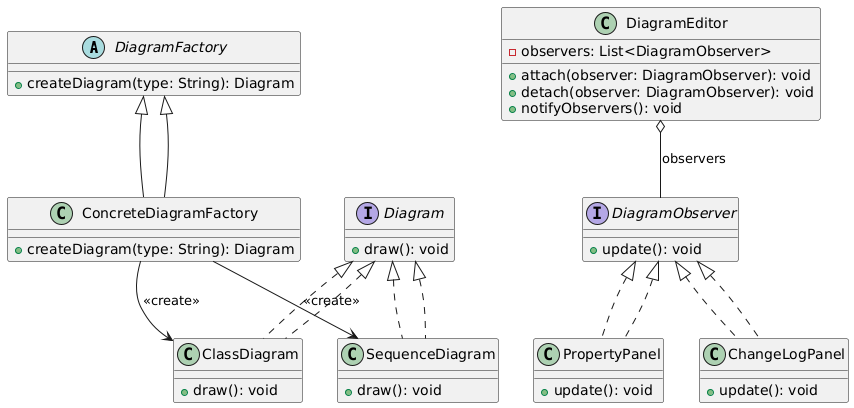
\includegraphics[width=\columnwidth]{1}
    	\caption{Діаграма класів}
    \end{figure}
    
    \begin{lstlisting}
    	class DiagramFactory {
    		createDiagram(type) {
    			throw "Method not implemented.";
    		}
    	}
    	
    	class ConcreteDiagramFactory extends DiagramFactory {
    		createDiagram(type) {
    			switch (type) {
    				case "class":
    				return new ClassDiagram();
    				case "sequence":
    				return new SequenceDiagram();
    				default:
    				throw "Unknown diagram type";
    			}
    		}
    	}
    	
    	class Diagram {
    		draw() {
    			throw "Method not implemented.";
    		}
    	}
    	
    	class ClassDiagram extends Diagram {
    		draw() {
    			console.log("Drawing Class Diagram");
    		}
    	}
    	
    	class SequenceDiagram extends Diagram {
    		draw() {
    			console.log("Drawing Sequence Diagram");
    		}
    	}
    	
    	const factory = new ConcreteDiagramFactory();
    	const diagram = factory.createDiagram("class");
    	diagram.draw();
    	
    \end{lstlisting}
    
    \begin{lstlisting}
    	class DiagramEditor {
    		constructor() {
    			this.observers = [];
    		}
    		
    		attach(observer) {
    			this.observers.push(observer);
    		}
    		
    		detach(observer) {
    			this.observers = this.observers.filter(obs => obs !== observer);
    		}
    		
    		notifyObservers() {
    			this.observers.forEach(observer => observer.update());
    		}
    		
    		change() {
    			console.log("Diagram changed");
    			this.notifyObservers();
    		}
    	}
    	
    	class DiagramObserver {
    		update() {
    			throw "Method not implemented.";
    		}
    	}
    	
    	class PropertyPanel extends DiagramObserver {
    		update() {
    			console.log("Property Panel updated");
    		}
    	}
    	
    	class ChangeLogPanel extends DiagramObserver {
    		update() {
    			console.log("Change Log updated");
    		}
    	}
    	
    	const editor = new DiagramEditor();
    	const propertyPanel = new PropertyPanel();
    	const changeLogPanel = new ChangeLogPanel();
    	
    	editor.attach(propertyPanel);
    	editor.attach(changeLogPanel);
    	
    	editor.change();
    	
    \end{lstlisting}
    
	\section*{Висновки}
	У ході виконання лабораторної роботи ми ознайомилися з основними шаблонами проектування, навчилися застосовувати їх при проектуванні і розробці ПЗ.

	    
\end{normalsize}
\end{document}
